\lecture

\begin{guiding}
Stiefel--Whitney numbers are computable invariants of closed manifolds. Which
equivalence relation do they detect? And is there a universal space from which
\emph{all} characteristic classes originate?
\end{guiding}

\section{Stiefel--Whitney numbers and cobordism}

\begin{example}\label{ex:odd-RP-numbers}
All Stiefel--Whitney numbers of $\RP^{2n-1}$ vanish.

Indeed $w(T\RP^{2n-1})=(1+a)^{2n}=(1+a^2)^n$ contains only terms of even degree,
so $w_i(T\RP^{2n-1})=0$ whenever $i$ is odd. A monomial
$w_1^{r_1}\cdots w_{2n-1}^{r_{2n-1}}$ of total degree $\sum i\,r_i=2n-1$ must
have $i\,r_i$ odd for at least one $i$, hence both $i$ and $r_i$ odd; that
factor is $w_i^{r_i}=0$.
\end{example}

\begin{theorem}\label{thm:boundary-numbers-vanish}
If $M^n$ is the boundary of a compact smooth $(n+1)$-manifold $B$, then all
Stiefel--Whitney numbers of $M$ vanish.
\end{theorem}

\begin{proof}
\begin{strategy}
The tangent bundle of $M$ is the restriction of the tangent bundle of $B$, up to
a trivial summand, so every characteristic class of $M$ in top degree is
restricted from $B$. On the other hand the fundamental class of $M$ is the
boundary of the fundamental class of $B$, and the evaluation pairing turns
$\partial$ into $\delta$. Exactness of the sequence of the pair kills the
result.
\end{strategy}

\step{1} \emph{Classes come from $B$.} Along $M=\partial B$ there is a
well-defined outward pointing direction, giving a nowhere zero section of
$TB|_M$ transverse to $TM$, hence a trivial line sub-bundle $\eps^1$ with
\[
TB|_M\ \iso\ TM\oplus\eps^1 .
\]
By Proposition~\ref{prop:stability} and naturality, for the inclusion
$i\colon M\hookrightarrow B$,
\[
i^*w_j(TB)=w_j\big(TB|_M\big)=w_j(TM).
\]

\step{2} \emph{Fundamental classes.} With $\Z_2$ coefficients,
$H_{n+1}(B,M;\Z_2)$ contains the fundamental class $\mu_B$ of the compact
manifold with boundary, and the connecting homomorphism of the pair sends
\[
\partial\colon H_{n+1}(B,M;\Z_2)\longrightarrow H_n(M;\Z_2),
\qquad
\mu_B\longmapsto\mu_M .
\]

\step{3} \emph{Transferring the evaluation.} Let
$v=w_1(TB)^{r_1}\smile\cdots\smile w_n(TB)^{r_n}\in H^n(B;\Z_2)$ with
$\sum i\,r_i=n$. By Step 1, $i^*v$ is the corresponding monomial in the classes
of $TM$. Using Step 2 and the definition of the connecting maps,
\[
\big\langle i^*v,\ \mu_M\big\rangle
=\big\langle i^*v,\ \partial\mu_B\big\rangle
=\big\langle \delta\,i^*v,\ \mu_B\big\rangle .
\]

\step{4} \emph{Exactness.} The cohomology sequence of the pair $(B,M)$ contains
\[
H^n(B;\Z_2)\ \xrightarrow{\ i^*\ }\ H^n(M;\Z_2)
\ \xrightarrow{\ \delta\ }\ H^{n+1}(B,M;\Z_2),
\]
so $\delta\circ i^*=0$. Hence the expression in Step 3 vanishes, and every
Stiefel--Whitney number of $M$ is zero.
\end{proof}

\begin{center}
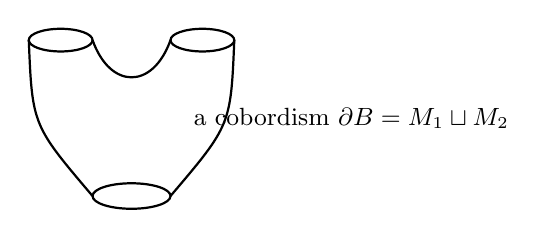
\begin{tikzpicture}[scale=0.9]
\draw[thick] (0,0) ellipse (0.45 and 0.16);
\draw[thick] (2,0) ellipse (0.45 and 0.16);
\draw[thick] (1,-2.2) ellipse (0.55 and 0.18);
\draw[thick] (-0.45,0) .. controls (-0.4,-1.2) .. (0.45,-2.2);
\draw[thick] (2.45,0) .. controls (2.4,-1.2) .. (1.55,-2.2);
\draw[thick] (0.45,0) .. controls (0.7,-0.7) and (1.3,-0.7) .. (1.55,0);
\node at (4.1,-1.1) {\small a cobordism $\partial B=M_1\sqcup M_2$};
\end{tikzpicture}
\end{center}

\begin{theorem}[Thom; quoted without proof]
Conversely, if all Stiefel--Whitney numbers of a closed smooth manifold $M$
vanish, then $M$ is a boundary.
\end{theorem}

This converse is genuinely hard; it is proved by the cobordism machinery
sketched in Lecture 12. See Milnor--Stasheff, \S 4 and \S 18, or Thom's original
paper.

\begin{definition}
Two closed smooth $n$-manifolds $M_1,M_2$ are \emph{(unoriented) cobordant} if
there is a compact smooth manifold $B$ with $\partial B=M_1\sqcup M_2$.
\end{definition}

\begin{corollary}
Two closed smooth manifolds are cobordant if and only if their
Stiefel--Whitney numbers are equal. In particular the numbers determine the
unoriented cobordism class.
\end{corollary}

\begin{proof}
If they are cobordant, Theorem~\ref{thm:boundary-numbers-vanish} applied to
$M_1\sqcup M_2$ gives $w_I[M_1]+w_I[M_2]=0$ for every partition $I$, hence
equality since we work mod $2$. Conversely, if the numbers agree then all
numbers of $M_1\sqcup M_2$ vanish and Thom's theorem makes $M_1\sqcup M_2$ a
boundary, that is, a cobordism between $M_1$ and $M_2$.
\end{proof}

\section{Classifying spaces}

\begin{guiding}
Where do characteristic classes come from? The slogan to aim at: bundles over
$B$ are the same thing as homotopy classes of maps from $B$ to one fixed
universal space, so that every cohomology class of that space produces an
invariant of bundles.
\end{guiding}

Recall that a \emph{fibre bundle} $(\pi,E,B,F)$ is a continuous surjection
$\pi\colon E\to B$ with local trivializations $U\times F\iso\pi^{-1}(U)$, and
that a \emph{principal $G$-bundle} is a fibre bundle carrying a $G$-action which
preserves the fibres and is free and transitive on each of them, so that each
fibre is homeomorphic to $G$.

Given a topological group $G$ there is a contractible space $EG$ on which $G$
acts freely; the quotient map
\[
\pi\colon EG\longrightarrow BG=EG/G
\]
is the \emph{universal principal $G$-bundle}, and $BG$ is the \emph{classifying
space}. We quote the following.

\begin{theorem}[quoted]
If $M$ is paracompact and $P\to M$ is a principal $G$-bundle, then there is a
map $f\colon M\to BG$ with $f^*EG\iso P$.
\end{theorem}

For vector bundles the relevant group is $\GL_n(\R)$, or $\Or(n)$ in the
presence of a Euclidean metric: to an $\R^n$-bundle one associates its
\emph{frame bundle}, the principal $\GL_n(\R)$-bundle whose fibre over $b$ is
the set of frames of $F_b(\xi)$; orthonormal frames give a principal
$\Or(n)$-bundle. Conversely a principal bundle $P$ recovers the vector bundle
$P\times_{\GL_n}\R^n$. So the classifying space we want is $B\Or(n)$, and it has
a concrete model: the Grassmannian, with $E\Or(n)$ modelled on a Stiefel
manifold.

\section{Grassmannians and universal bundles}

The motivation is geometric. A curve $C\subset\R^{k+1}$ has a tangent line at
each point, giving a map $C\to\RP^k$; an $n$-manifold $M\subset\R^{n+k}$ has a
tangent $n$-plane at each point, giving a map to the space of all $n$-planes.

\begin{definition}
The \emph{Grassmann manifold} $G_n(\R^{n+k})$ is the set of $n$-dimensional
linear subspaces of $\R^{n+k}$. In particular $G_1(\R^{k+1})=\RP^k$.
\end{definition}

\begin{definition}
An \emph{$n$-frame} in $\R^{n+k}$ is an $n$-tuple of linearly independent
vectors. The \emph{Stiefel manifold} $V_n(\R^{n+k})\subset(\R^{n+k})^n$ is the
set of $n$-frames, an open subset since it is
$\{A\mid\det AA^{\mathsf T}\neq0\}$, the preimage of $\R\smallsetminus\{0\}$
under a continuous map. Let $V_n^0(\R^{n+k})\subset V_n(\R^{n+k})$ be the
subspace of \emph{orthonormal} frames.
\end{definition}

We topologize $G_n(\R^{n+k})$ as the quotient of $V_n(\R^{n+k})$ under
$q=\spann$.

\begin{proposition}
$G_n(\R^{n+k})$ is compact.
\end{proposition}

\begin{proof}
The set $V_n^0(\R^{n+k})$ is closed and bounded in $(\R^{n+k})^n$ --- it is cut
out by the equations $x_i\cdot x_j=\delta_{ij}$ --- hence compact. Gram--Schmidt
is a continuous retraction $V_n\to V_n^0$ commuting with $q$, so
$q|_{V_n^0}\colon V_n^0\to G_n(\R^{n+k})$ is onto. A continuous image of a
compact space is compact.
\end{proof}

\begin{theorem}\label{thm:grassmannian-manifold}
$G_n(\R^{n+k})$ is a topological manifold of dimension $nk$, and
$X\mapsto X^\perp$ is a homeomorphism
$G_n(\R^{n+k})\iso G_k(\R^{n+k})$.
\end{theorem}

\begin{proof}
\begin{strategy}
Hausdorffness is proved by separating two planes with an explicit continuous
function, namely the distance to a vector lying in one and not the other.
Charts come from the observation that the planes close to a fixed $X_0$ are
exactly the graphs of linear maps $X_0\to X_0^\perp$; the identification with
$\Hom(X_0,X_0^\perp)$ is the chart.
\end{strategy}

\step{1} \emph{A supply of continuous functions.} For $w\in\R^{n+k}$ let
$\rho_w(X)$ be the squared distance from $w$ to the plane $X$. If
$(x_1,\dots,x_n)$ is an orthonormal frame of $X$ then
\[
\rho_w(X)=w\cdot w-(w\cdot x_1)^2-\dots-(w\cdot x_n)^2,
\]
which is continuous in the frame. Hence $\rho_w\circ q$ is continuous on
$V^0_n$, and since $G_n$ carries the quotient topology, $\rho_w$ is continuous
on $G_n(\R^{n+k})$.

\step{2} \emph{Hausdorff.} Let $X_1\neq X_2$ and choose
$w\in X_1\smallsetminus X_2$. Then $\rho_w(X_1)=0$ while $\rho_w(X_2)>0$, so the
preimages under $\rho_w$ of two disjoint intervals separate $X_1$ from $X_2$.

\step{3} \emph{The chart domain.} Fix $X_0$ and split
$\R^{n+k}=X_0\oplus X_0^{\perp}$. Let
\[
U=\big\{Y\in G_n(\R^{n+k})\ \big|\
\proj_{X_0}\!\big|_Y\colon Y\to X_0 \text{ is an isomorphism}\big\}
\]
that is, $U=\{Y\mid Y\cap X_0^{\perp}=0\}$. This is
an open neighbourhood of $X_0$: writing $Y=q(y_1,\dots,y_n)$, the condition is
that a certain determinant in the frame be non-zero.

\step{4} \emph{The chart.} For $Y\in U$ every element of $Y$ is determined by
its $X_0$-component, so $Y$ is the graph
\[
Y=\big\{\,x+T(Y)x\ \big|\ x\in X_0\,\big\}
\]
of a unique linear map $T(Y)\colon X_0\to X_0^\perp$. This gives a bijection
\[
T\colon U\longrightarrow\Hom(X_0,X_0^\perp)\iso\R^{nk}.
\]

\step{5} \emph{Continuity both ways.} Choose an orthonormal basis
$x_1,\dots,x_n$ of $X_0$. For $Y\in U$ the vectors $y_i=x_i+T(Y)x_i$ form a
frame of $Y$, and conversely any frame of $Y$ close to that of $X_0$ can be
normalized to this form by an invertible linear change, depending continuously
on the frame. Hence $y_i$ depends continuously on $Y$ and vice versa, and
$T(Y)$ is determined by the $y_i$ through $T(Y)x_i=y_i-x_i$. So both $T$ and
$T^{-1}$ are continuous, and $U\iso\R^{nk}$.

\step{6} \emph{The duality homeomorphism.} The assignment $Y\mapsto Y^{\perp}$
is a bijection $G_n(\R^{n+k})\to G_k(\R^{n+k})$, and it is continuous: an
orthonormal frame of $Y$ can be completed continuously, locally in $Y$, to an
orthonormal frame of $\R^{n+k}$ by the Gram--Schmidt argument of
Theorem~\ref{thm:orthogonal-complement}, and the last $k$ vectors give a frame
of $Y^\perp$. Applying the same to $Y^\perp$ gives continuity of the inverse.
\end{proof}

\begin{definition}
The \emph{tautological bundle} $\gamma^n(\R^{n+k})$ over $G_n(\R^{n+k})$ has
total space
\[
E=\big\{(X,\vec v)\ \big|\ X\in G_n(\R^{n+k}),\ \vec v\in X\big\}
\]
and projection $(X,\vec v)\mapsto X$. For $n=1$ this is
$\gamma^1(\R^{k+1})=\gamma^1_k\to\RP^k$.
\end{definition}

\begin{lemma}\label{lem:tautological-locally-trivial}
$\gamma^n(\R^{n+k})$ is locally trivial, hence a vector bundle of rank $n$.
\end{lemma}

\begin{proof}
Work over the chart domain $U$ of $X_0$ from Step 3 above. For $Y\in U$ the
orthogonal projection $P_Y\colon Y\to X_0$ is an isomorphism, so we may define
\[
h\colon U\times X_0\longrightarrow\pi^{-1}(U),
\qquad
h(Y,x)=\big(Y,\ P_Y^{-1}(x)\big)=\big(Y,\ x+T(Y)x\big).
\]
By Step 5 of Theorem~\ref{thm:grassmannian-manifold} the map $T$ is continuous,
so $h$ is continuous; its inverse is $(Y,v)\mapsto(Y,\proj_{X_0}v)$, also
continuous; and for fixed $Y$ it is a linear isomorphism $X_0\to Y$. Identifying
$X_0\iso\R^n$ gives a local trivialization.
\end{proof}

\begin{definition}
For a smooth $M^n\subset\R^{n+k}$, the \emph{generalized Gauss map} is
\[
\bar g\colon M\longrightarrow G_n(\R^{n+k}),
\qquad
x\longmapsto T_xM,
\]
the base map of the bundle map
$g\colon TM\to\gamma^n(\R^{n+k})$, $(x,v)\mapsto(T_xM,v)$.
\end{definition}

So tangent bundles of submanifolds of Euclidean space are pulled back from
tautological bundles. The following says this is neither an accident nor a
restriction.

\begin{lemma}\label{lem:compact-classify}
Let $\xi$ be an $\R^n$-bundle over a \emph{compact} base $B$. Then for $k$ large
enough there is a bundle map $\xi\to\gamma^n(\R^{n+k})$.
\end{lemma}

\begin{proof}
\begin{strategy}
A bundle map into a tautological bundle is the same thing as a map from the
total space to a Euclidean space, linear and injective on each fibre; the plane
component of the bundle map is then forced. Such a map is assembled from
finitely many local trivializations, damped by bump functions so that they
extend by zero, and stacked into a single large Euclidean space.
\end{strategy}

\step{1} \emph{Reduction.} Suppose we have a continuous
$\hat f\colon E(\xi)\to\R^m$ which is linear and injective on every fibre. Then
\[
f(e)=\Big(\ \hat f\big(F_{\pi(e)}(\xi)\big),\ \hat f(e)\ \Big)
\]
defines a map $E(\xi)\to E\big(\gamma^n(\R^m)\big)$: the first entry is an
$n$-plane in $\R^m$ because $\hat f$ is injective and linear on the fibre, and
the second lies in it. It is fibrewise a linear isomorphism onto that plane. Its
continuity follows from the continuity of $\hat f$ together with the local
description of the chart in Lemma~\ref{lem:tautological-locally-trivial}.

\step{2} \emph{Bump functions.} By compactness choose a finite trivializing
cover $U_1,\dots,U_r$ of $B$, sets $W_i\subset\overline{W_i}\subset V_i\subset
\overline{V_i}\subset U_i$ with $\{W_i\}$ still covering $B$, and continuous
$\lambda_i\colon B\to[0,1]$ with $\lambda_i=1$ on $W_i$ and $\lambda_i=0$
outside $V_i$.

\step{3} \emph{Damped local coordinates.} Each trivialization
$h_i\colon U_i\times\R^n\to\pi^{-1}(U_i)$ gives
$\tilde h_i=\proj_{\R^n}\circ\,h_i^{-1}\colon\pi^{-1}(U_i)\to\R^n$, linear and
injective on each fibre over $U_i$. Define
\[
h'_i\colon E(\xi)\longrightarrow\R^n,
\qquad
h'_i(e)=\lambda_i\big(\pi(e)\big)\cdot\tilde h_i(e)
\]
for $\pi(e)\in U_i$, and $h'_i(e)=0$ otherwise. This is continuous: the two
definitions agree on the overlap $U_i\smallsetminus \overline{V_i}$, where
$\lambda_i=0$.

\step{4} \emph{Stacking.} Set $m=rn$ and
\[
\hat f=(h'_1,\dots,h'_r)\colon E(\xi)\longrightarrow
\underbrace{\R^n\oplus\dots\oplus\R^n}_{r}=\R^{m}.
\]
It is continuous and linear on fibres. It is injective on the fibre over $b$:
some $W_i$ contains $b$, so $\lambda_i(b)=1$ and the $i$-th component is
$\tilde h_i$, already injective there.

\step{5} By Step 1 this $\hat f$ produces a bundle map
$\xi\to\gamma^n(\R^{m})$, and $m=rn$ is of the form $n+k$ with $k=(r-1)n$.
\end{proof}

To remove the dependence on $k$, let $\R^\infty=\bigcup_m\R^m$ carry the direct
limit topology and define the \emph{infinite Grassmannian}
\[
G_n=G_n(\R^\infty)=\varinjlim_k G_n(\R^{n+k}),
\]
with tautological bundle $\gamma^n$ defined by the same formula. This is the
\emph{universal $n$-plane bundle}. In the next lecture we prove that every
$\R^n$-bundle over a paracompact base admits a bundle map to $\gamma^n$, unique
up to homotopy, so that
\[
\big\{\R^n\text{-bundles over }B\big\}\big/\!\iso
\ \ \longleftrightarrow\ \
\big[\,B,\ G_n\,\big],
\]
and characteristic classes are then simply elements of $H^*(G_n)$ pulled back
along classifying maps.
